\documentclass{article}

% Margin definition.
\usepackage[a4paper,total={6.8in, 8.5in}]{geometry}
\usepackage{parskip}
\usepackage[bottom]{footmisc}
% Images.
\usepackage{graphicx}
\usepackage[export]{adjustbox}
\usepackage{float}
% Table
\usepackage{array}
\usepackage[toc,page]{appendix}
% Links.
\usepackage[T1,hyphens]{url}
\usepackage[hidelinks, bookmarks=true]{hyperref}
% Encoding.
\usepackage[utf8]{inputenc}
% Helvetic font.
\usepackage[scaled]{helvet}
\renewcommand\familydefault{\sfdefault} 
% Header for ua logo.
\usepackage{fancyhdr}
% Dots in index.
\usepackage[titles]{tocloft}
\renewcommand{\cftsubsubsecleader}{\Large\cftdotfill{0}}
\renewcommand{\cftsubsecleader}{\Large\cftdotfill{0}}
\renewcommand{\cftsecleader}{\Large\cftdotfill{0}}
\renewcommand{\cftsecfont}{\large\bfseries\scshape}
\renewcommand{\cftsubsecfont}{\scshape}
\renewcommand{\cftsubsubsecfont}{\small\scshape}
\addtolength{\cftsecnumwidth}{5pt}
\renewcommand*{\HyperDestNameFilter}[1]{\jobname-#1}
% Dot after number in (sub)sections and in toc.
\renewcommand{\cftsecaftersnum}{.}
\renewcommand{\cftsubsecaftersnum}{}
\usepackage[letterspace=45]{microtype}
\newcommand*{\fullref}[1]{\hyperref[{#1}]{\autoref*{#1} \nameref*{#1} \urlref*{#1}}}
% Header with ua logo definition. 
\pagestyle{fancy}
\fancyhf{}
\chead{
    
\includegraphics[height=0.5in]{./img/header_ua.png}
}
\setlength\headheight{45pt}
% Footer with page number.
\rfoot{Page \thepage}
\renewcommand{\footrulewidth}{0.4pt}
% Rename table of contents title to "Index"
% \renewcommand{\contentsname}{\Large Index \vspace{0.3cm}}

% for code
\usepackage{listings}
\lstset{
  basicstyle=\ttfamily,
  columns=fullflexible,
  frame=single,
  breaklines=true,
  postbreak=\mbox{\textcolor{red}{$\hookrightarrow$}\space},
}
\usepackage{xcolor}

\usepackage{hyperref}
\hypersetup{
    colorlinks=true,
    linkcolor=blue,
    filecolor=magenta,      
    urlcolor=cyan,
}

\definecolor{codegreen}{rgb}{0,0.6,0}
\definecolor{codegray}{rgb}{0.5,0.5,0.5}
\definecolor{codepurple}{rgb}{0.58,0,0.82}
\definecolor{backcolour}{rgb}{0.95,0.95,0.92}

\lstdefinestyle{mystyle}{
    backgroundcolor=\color{backcolour},   
    commentstyle=\color{codegreen},
    keywordstyle=\color{magenta},
    numberstyle=\tiny\color{codegray},
    stringstyle=\color{codepurple},
    basicstyle=\ttfamily\footnotesize,
    breakatwhitespace=false,         
    breaklines=true,                 
    captionpos=b,                    
    keepspaces=true,                 
    numbers=left,                    
    numbersep=5pt,                  
    showspaces=false,                
    showstringspaces=false,
    showtabs=false,                  
    tabsize=2,
    inputencoding=utf8
}

\lstset{style=mystyle}

\usepackage{float}
\usepackage{subfig}


% for the references
\usepackage[nottoc,numbib]{tocbibind}

% section on new page, except the index one
\usepackage{etoolbox}
\pretocmd{\section}{%
  \ifnum\value{section}=0 \else\clearpage\fi
}{}{}


%encoding
%--------------------------------------
\usepackage[T1]{fontenc}
\usepackage[utf8]{inputenc}
%--------------------------------------

%Portuguese-specific commands
%--------------------------------------
% \usepackage[portuguese]{babel}
%--------------------------------------

%Hyphenation rules
%--------------------------------------
\usepackage{hyphenat}
\hyphenation{mate-mática recu-perar}
%--------------------------------------

\usepackage{mathtools}
\usepackage{makecell}


\makeatletter
\renewcommand{\maketitle}{\bgroup\setlength{\parindent}{10pt}
\begin{flushleft}
  \textbf{\Huge \@title}

  \large{\textbf{\@author}}\\
  \vspace{0.3cm}
  \normalsize{\@date}\\
\end{flushleft}\egroup
}
\makeatother
\title{Gestão de identidades centradas no utente}
\author{Rafael José Santos Simões\\\normalsize{rafaeljsimoes@ua.pt}}
\date{26/06/2021}


\begin{document}

\maketitle
\vspace{1cm}

\thispagestyle{empty}


\tableofcontents

\newpage

\fontsize{12pt}{13pt}
\selectfont
\lsstyle

\section{Introdução}


\quad Este projeto baseia-se numa mudança protocolar relativamente ao primeiro projeto desta cadeira. Neste caso, o objetivo é o utilizador ter controlo ativo sobre os atributos de entidade usados durante os processos de autenticação, isto é, este tem plena noção que atributos de identidade estão a ser requisitados (por um  \textit{Service provider} (SP)) e o resultado da sua resolução (providenciado por um \textit{identity provider} (IDP)). Complementarmente à amostrem explicita dos atributos de entidades, o utilizador consegue tomar de decisões de consentimento (ou não) relativamente ao conjunto de atributos solicitados e resolvidos pelas entidades de autenticação. Outra caraterística vantajosa deste protocolo é a impossibilidade dos \textit{IDPs} conseguirem fazer \textit{track} de quais \textit{SPs} o utilizador interage.



\section{Formato usado para os pedidos e respostas de atributos de entidade}

\quad Sabendo que no primeiro projeto foi usado o padrão de troca de dados de autenticação e autorização entre entidades - \textbf{\textit{SAML}}, devido à natureza ativa do utilizador nos atributos de entidade e da flexibilidade na definição dos atributos de entidade a usar por parte do \textit{SP}, o padrão \textit{SAML} deixou de ser utilizável, uma vez que o \textit{SP} não consegue especificar os atributos de identidade (no pedido de autenticação)  que este necessita, pois isto é estabelecido pelo intercâmbio de meta-dados entre o \textit{SP} e o \textit{IDP} onde estes negoceiam a forma como vão interagir.\footnote{Apesar de não ser possível de utilizador o padrão SAML na totalidade, ainda é possível usar este padrão para o manuseamento de respostas de autenticação. Contudo, o padrão SAML foi completamente removido deste projeto, pois para possibilitar o uso deste padrão era necessário a \textit{helper application} interpretar pedidos usando o SAML (que não foi implementado no projeto 1)} Além disso, uma vez que as interações de \textit{SAML} eram apenas realizadas entre o \textit{IDP} e o \textit{SP}, os atributos de entidade usados poderiam nunca ser apresentados ao utilizador caso o \textit{IDP} não partilhasse essa informação.


\quad Como é expectável foi criado um novo formato de pedido e resposta para partilha de atributos de entidade.

\subsection{Formato do pedido de atributos de entidade}

\begin{itemize}
    \item \textbf{sp\_info}: Informação relativa ao \textit{SP}
    \begin{itemize}
        \item \textbf{id}: Valor que armazena o identificador do \textit{SP}
        \item \textbf{location}: \textit{URL} do \textit{SP} para receber os atributos pedidos e a respetiva assinatura
    \end{itemize}
    \item \textbf{identity\_attributes}: Lista de atributos requisitados pelo \textit{SP}
    \item \textbf{idp\_info}: Informação relativa ao \textit{IDP}
    \begin{itemize}
        \item \textbf{id}: Valor que armazena o identificador do \textit{IDP}
        \item \textbf{location}: \textit{URL} do \textit{IDP} que permite a obtenção dos atributos recebidos
    \end{itemize}
\end{itemize}


\begin{minipage}{\linewidth}
    \begin{lstlisting}[language=C, caption={Exemplo de um pedido de atributos de entidade}, label={lst:atribute_request}, escapeinside={(*}{*)}]
        {
            "sp_info": {
              "id": "http://localhost:8081",
              "location": "http://localhost:8081/receive_identity_attributes"
            },
            "identity_attributes": [
              "username",
              "email"
            ],
            "idp_info": {
              "id": "http://localhost:8082",
              "location": "http://localhost:8082/handle_identity_request"
            }
          }
    \end{lstlisting}
\end{minipage}

\subsection{Formato da resposta a um pedido de atributos de entidade}

\begin{itemize}
    \item \textbf{attributes}: Dicionário que armazena o mapeamento entre os atributos solicitados e o respetivo valor
    \item \textbf{signature}: Atributo que armazena a assinatura (em base64) dos atributos de entidade. Esta assinatura é realizada pelo \textit{IDP} usando a sua chave privada.
\end{itemize} 


\begin{minipage}{\linewidth}
    \begin{lstlisting}[language=C, caption={Exemplo da resposta ao pedido \ref{lst:atribute_request} de atributos de entidade}, label={lst:atribute_response}, escapeinside={(*}{*)}]
        {
            "attributes": {
              "username": "rafael",
              "email": "rafael@ua.pt"
            },
            "signature": "4UgFUEe+u3uauUnC2NzIbbzhe32p7rOdZCnTVaeynvvSIHEibasiozVv9nk0EsKo9Em4bqp0ms3WHrpC9C6gej
            SYvATUAO0IhVgVKX1mQnN3vgzJ1bCULa7rr7uVXxGL0N1domUPDuUdhjN8c32TB1CGBtI11G8qUQGfrn8APDc="
          }
    \end{lstlisting}
\end{minipage}
\section{Mudanças na arquitetura relativamente ao primeiro projeto}

\quad Como já foi referido, o utilizador tem poder ativo no que toca ao consentimento (ou não) no uso de atributos de entidade que lhe pertencem, por isso, o \textit{workflow} moldado à arquitetura do primeiro projeto terá que sofrer alterações para permitir que \textit{helper application} possa intercetar os pedidos e respostas de identificação para esta conseguir:

\begin{itemize}
    \item Apresentar ao utilizador que atributos de identidade foram requisitados pelo \textit{SP}
    \item Recolher o consentimento do utilizador e em caso positivo encaminhar o pedido de identidade para o \textit{IDP}
    \item Receber a resposta ao pedido de identidade, e apresentar ao utilizador que valores que foram devolvidos pelo \textit{IDP}
    \item Recolher o consentimento do utilizador sobre os valores recebidos e em caso positivo encaminhar a resposta ao pedido de identidade para o \textit{SP}.
\end{itemize}

\quad Como é fácil de perceber, a \textit{helper application} neste sistema, funciona como entidade central por onde todos os pedidos e respostas passam e a qualquer momento, devido a uma ação de não consentimento do utilizador, esta pode cancelar o \textit{workflow} deste protocolo cancelando quaisquer processos de identificação ativos.


\quad Uma das caraterísticas desta nova arquitetura é a necessidade de existir uma par de chaves assimétricas entre o utilizador (através da \textit{helper application}) e o \textit{IDP} para proceder ao protocolo de identificação. No projeto anterior, existiam dois métodos de autenticação, um através do protocolo \textit{ZKP} e outro usando um par de chaves assimétricas (geradas após um processo correto de autenticação usando o \textit{ZKP}), naquele caso as credenciais assimétricas serviram para melhorar o processo de autenticação em termos temporais uma vez que o processo de \textit{ZKP} é um processo consideravelmente lento. Neste projeto, o processo de autenticação com \textit{ZKP} vai continuar a existir, quer para autenticar o utilizador quer para gerar um par de chaves assimétricas. Após a criação do material criptográfico assimétrico é possível realizar o \textit{protocol collapsing} que num processo só permite realizar a autenticação do cliente e o fornecimento autenticado dos atributos de identidade. Portanto, qualquer explicação referente ao \textit{protocol collapsing} será inferido que já existe um par de chaves assimétricas após o \textit{ZKP}.


\subsection{\textit{Protocol collapsing}}

\quad Neste secção vai ser explicado o \textit{workflow} de operações necessários para realizar o processo de identificação de maneira segura neste serviço.


\begin{figure}[H]
    \caption{Protocolo de identificação usando o conceito de \textit{Protocol collapsing}}
    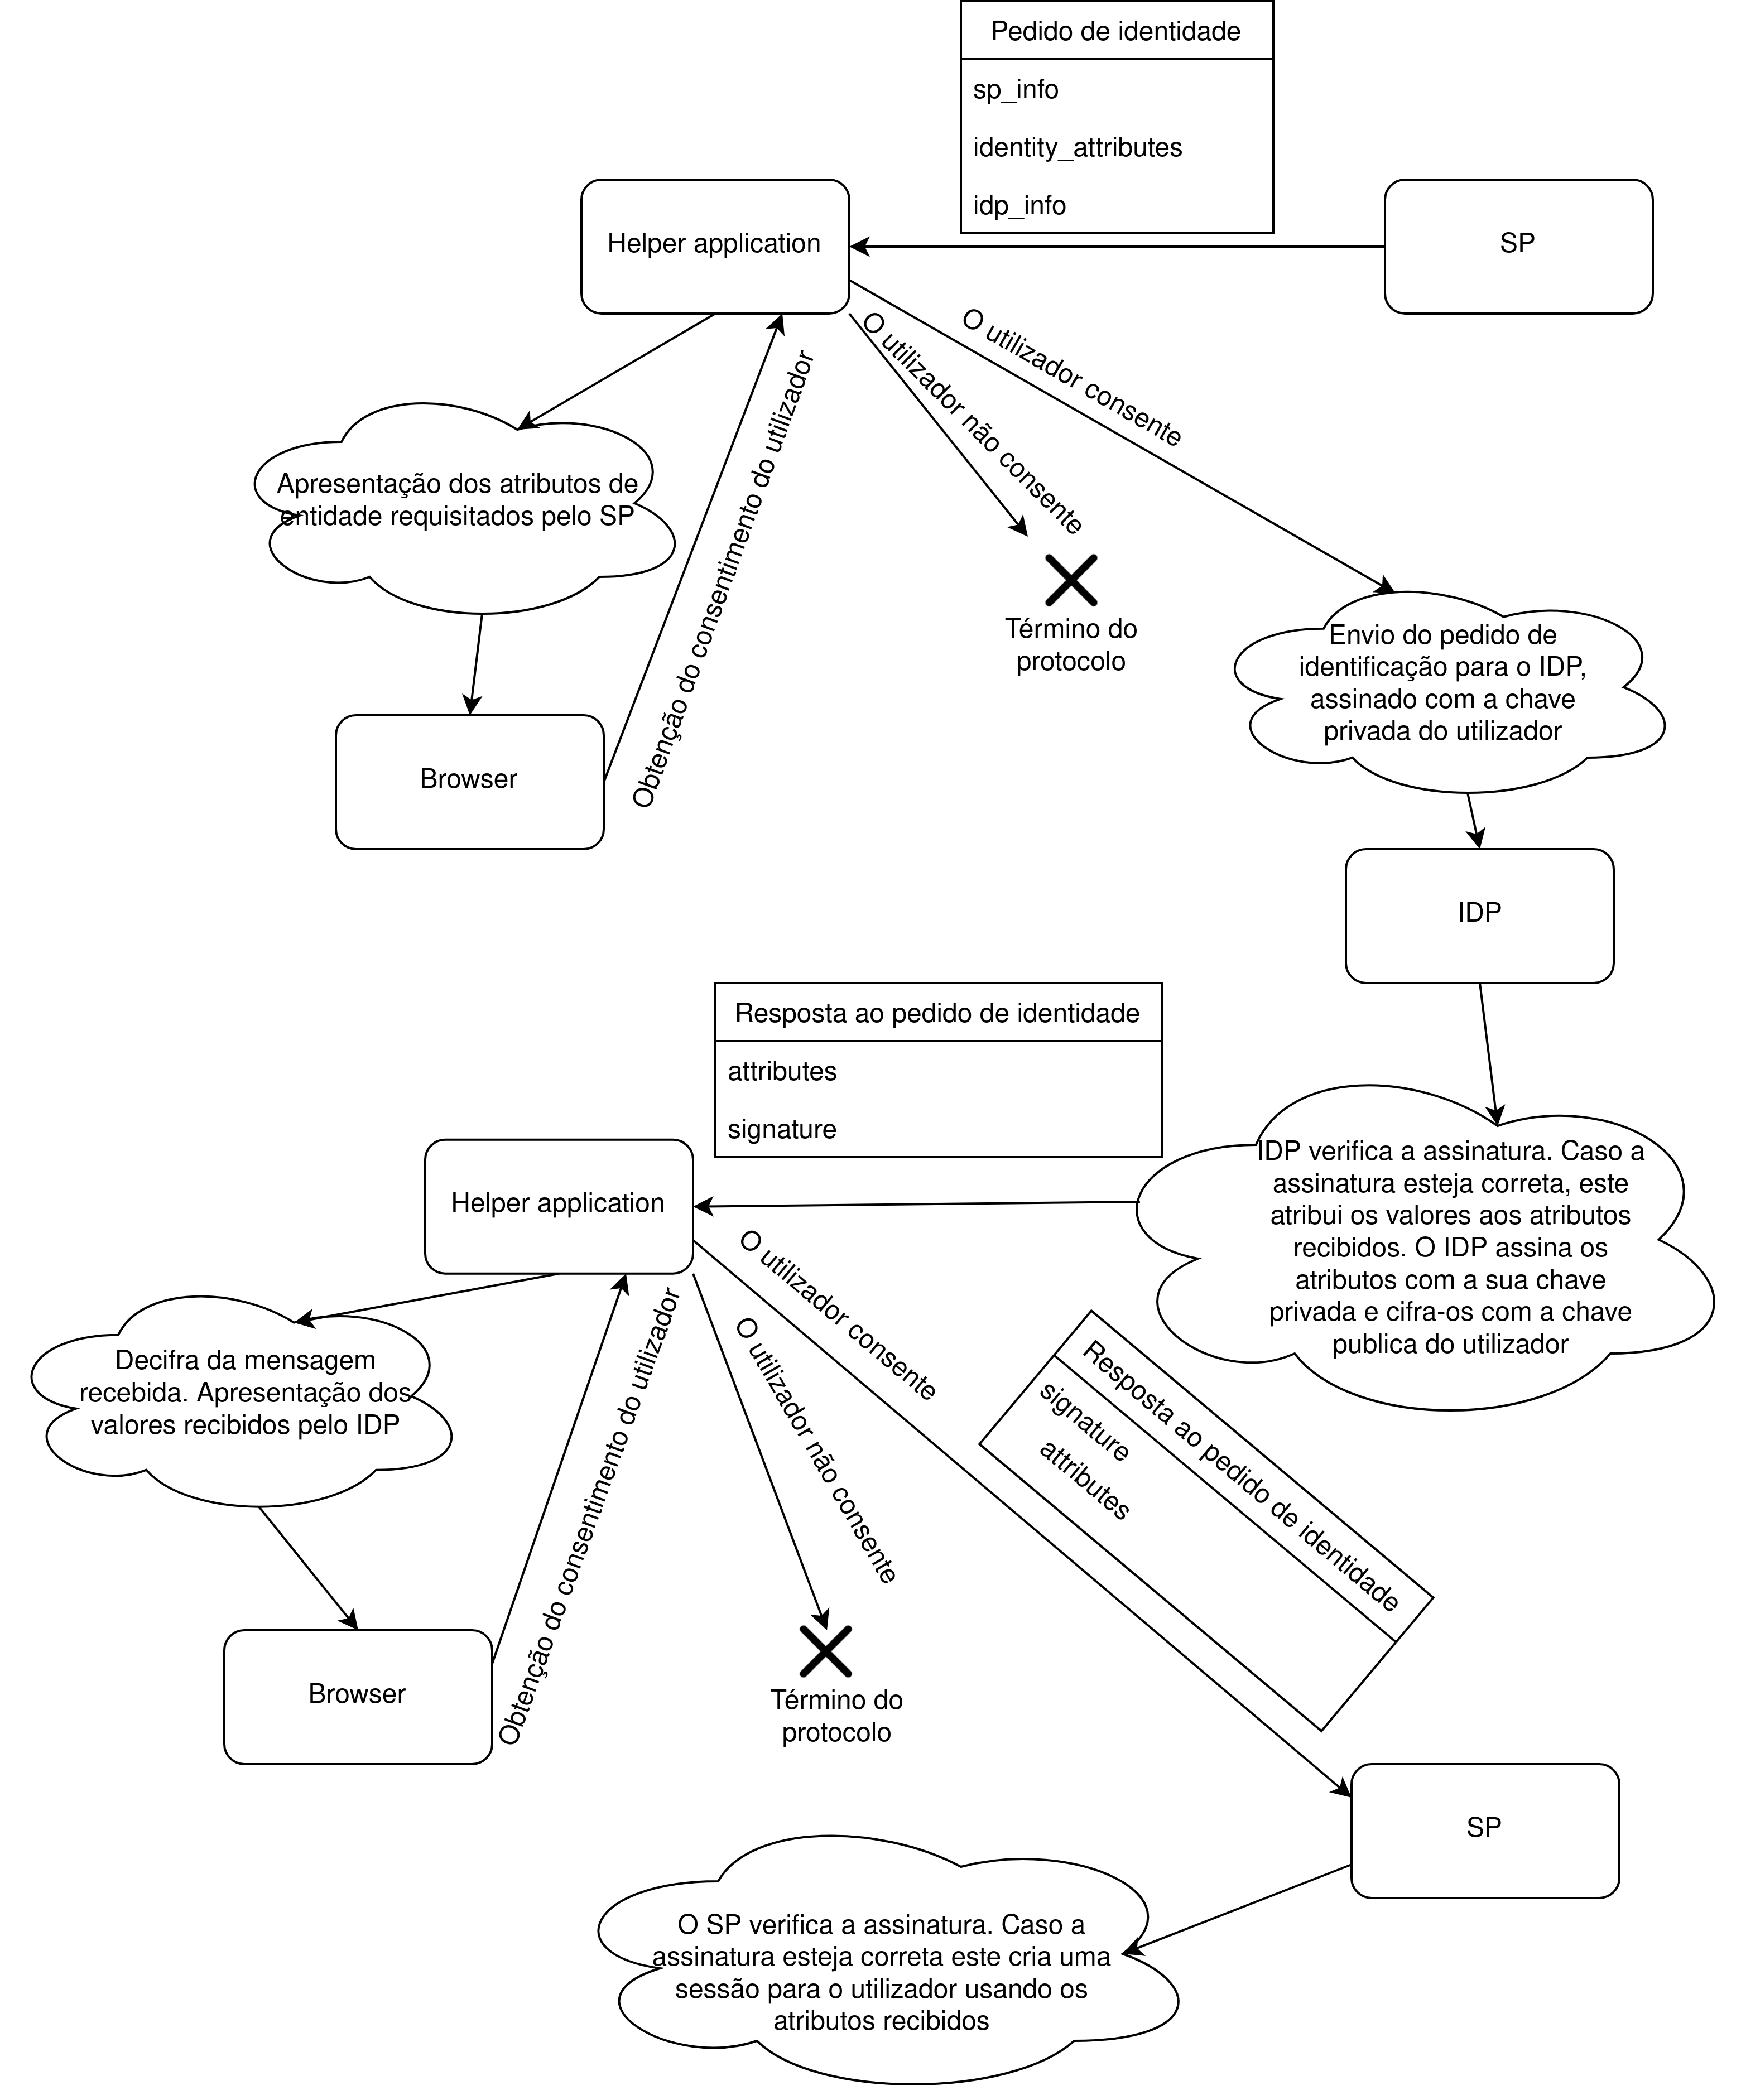
\includegraphics[width=\textwidth]{img/protocol_identity.png}
    \centering
\end{figure}


\begin{enumerate}
    \item O utilizador tenta aceder a um serviço disponibilizado por um \textit{SP} ao qual não tem uma sessão ativa, portanto, o \textit{SP} redireciona o utilizador para a \textit{helper application} enviando uma mensagem com os atributos de identidade necessários para criar uma sessão.
    \item A \textit{helper application} apresenta os atributos requisitados pelo \textit{SP} ao utilizador e obtém o consentimento do mesmo para conseguir enviar o pedido de identificação (com os atributos) para o \textit{IDP}. Obviamente, caso o utilizador não permita o uso dos atributos especificados a \textit{helper application} interrompe o processo e não envia o pedido para o \textit{IDP} \footnote{Neste fase é considerado que já existe um par de chaves assimétricas, caso estas não existam o utilizador deve ser autenticado com o protocolo \textit{ZKP} para de seguida serem criadas as credenciais assimétricas }
    \begin{figure}[H]
        \caption{Página mostrada pela \textit{helper application} para recolher o consentimento do utilizador antes do envio do pedido de identificação para o \textit{IDP}}
        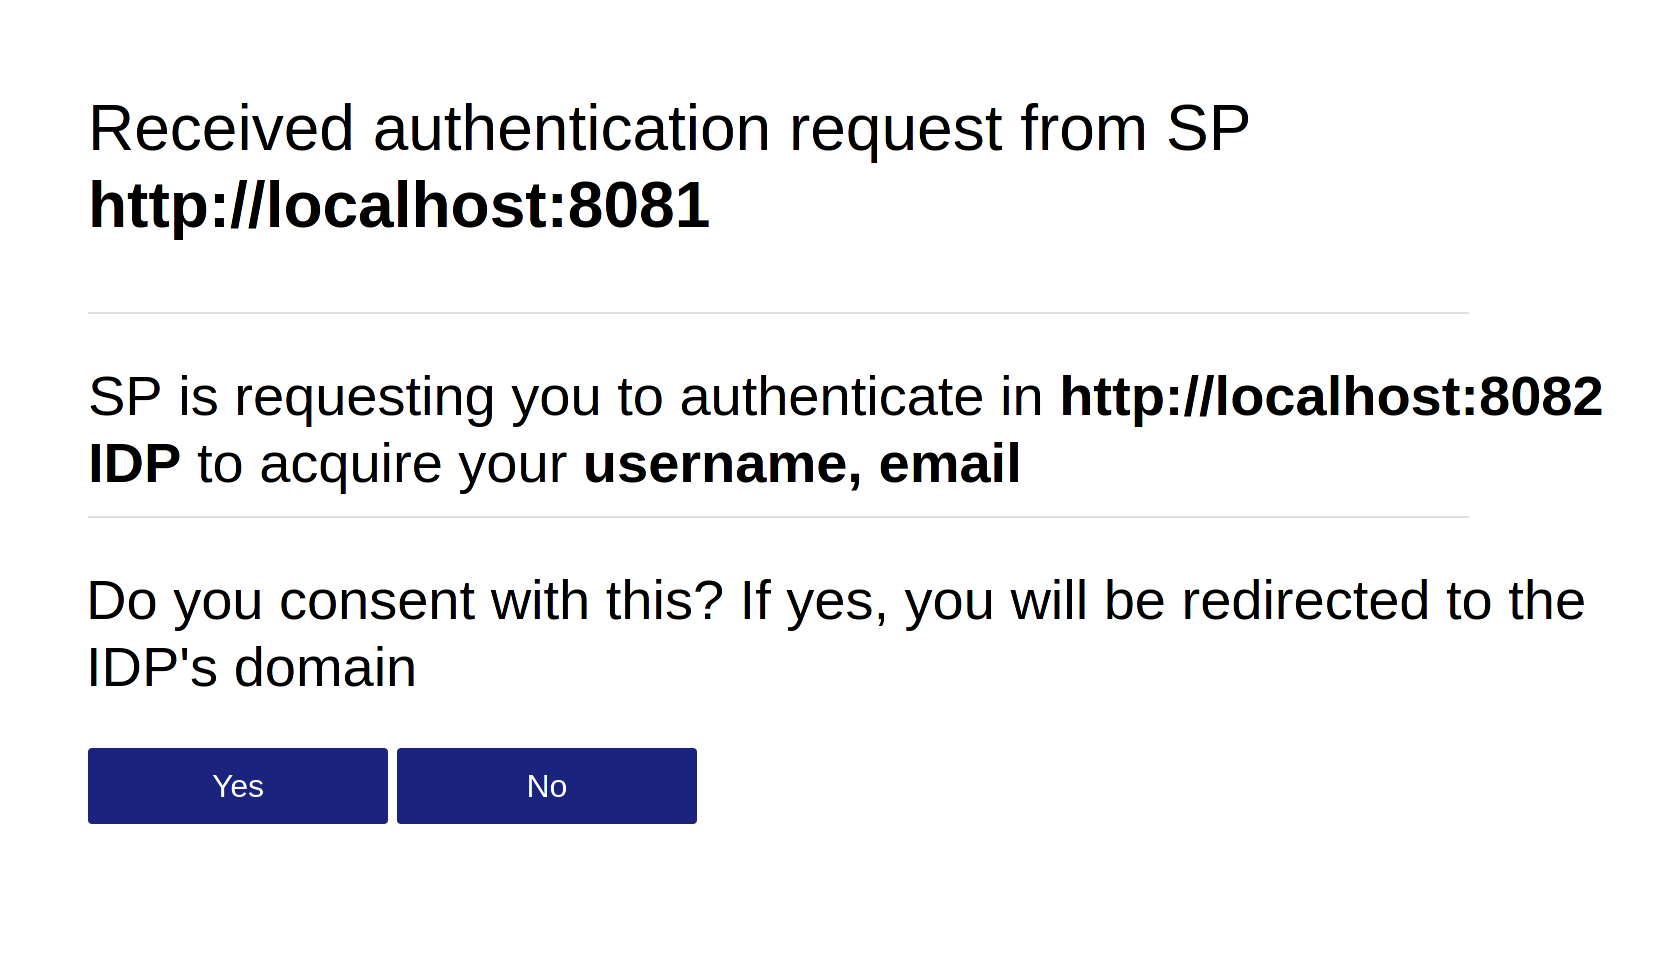
\includegraphics[width=0.6\textwidth]{img/request_conse.png}
        \centering
    \end{figure}
    \item Após receber o consentimento do utilizador a \textit{helper application} assina o pedido (usando a chave privada do utilizador, criada após o processo do \textit{ZKP}) de identificação (enviado pelo \textit{SP}) e envia o pedido e assinatura para o \textit{IDP}
    \item O \textit{IDP} após receber a mensagem anterior, este verifica a assinatura com o conteúdo recebido. Caso a assinatura seja válida este sabe que a mensagem veio do utilizador pretendido e que o conteúdo da mensagem não foi adulterado (daí o termo \textit{protocolo collapsing} pois permite numa verificação autenticar o utilizador e garantir que os dados não foram alterados no canal de comunicação). Depois da verificação da assinatura, o \textit{IDP} obtém os atributos necessários e encapsula-os numa nova mensagem com o mapeamento entre os atributos recebidos e os valores obtidos. Antes de enviar a resposta para a \textit{helper application} este faz uma assinatura sobre os conteúdos mapeados (com a chave privada associado ao \textit{IDP}) e cifra o conteúdo da mensagem com a chave publica do utilizador.
    \item A \textit{helper application} faz o processo de decifra (usando a chave privada do utilizador) da resposta recebida e apresenta ao utilizador os valores retornados pelo \textit{IDP}. Mais uma vez, obtém o consentimentos (ou não) do utilizador e caso este permita a \textit{helper application} envia o conteúdo da resposta e a respetiva assinatura para o \textit{SP}. Mais uma vez, caso não existe consentimento por parte do utilizador o processo é interrompido.
    \begin{figure}[H]
        \caption{Página mostrada pela \textit{helper application} para recolher o consentimento do utilizador antes do envio da resposta para o \textit{SP}}
        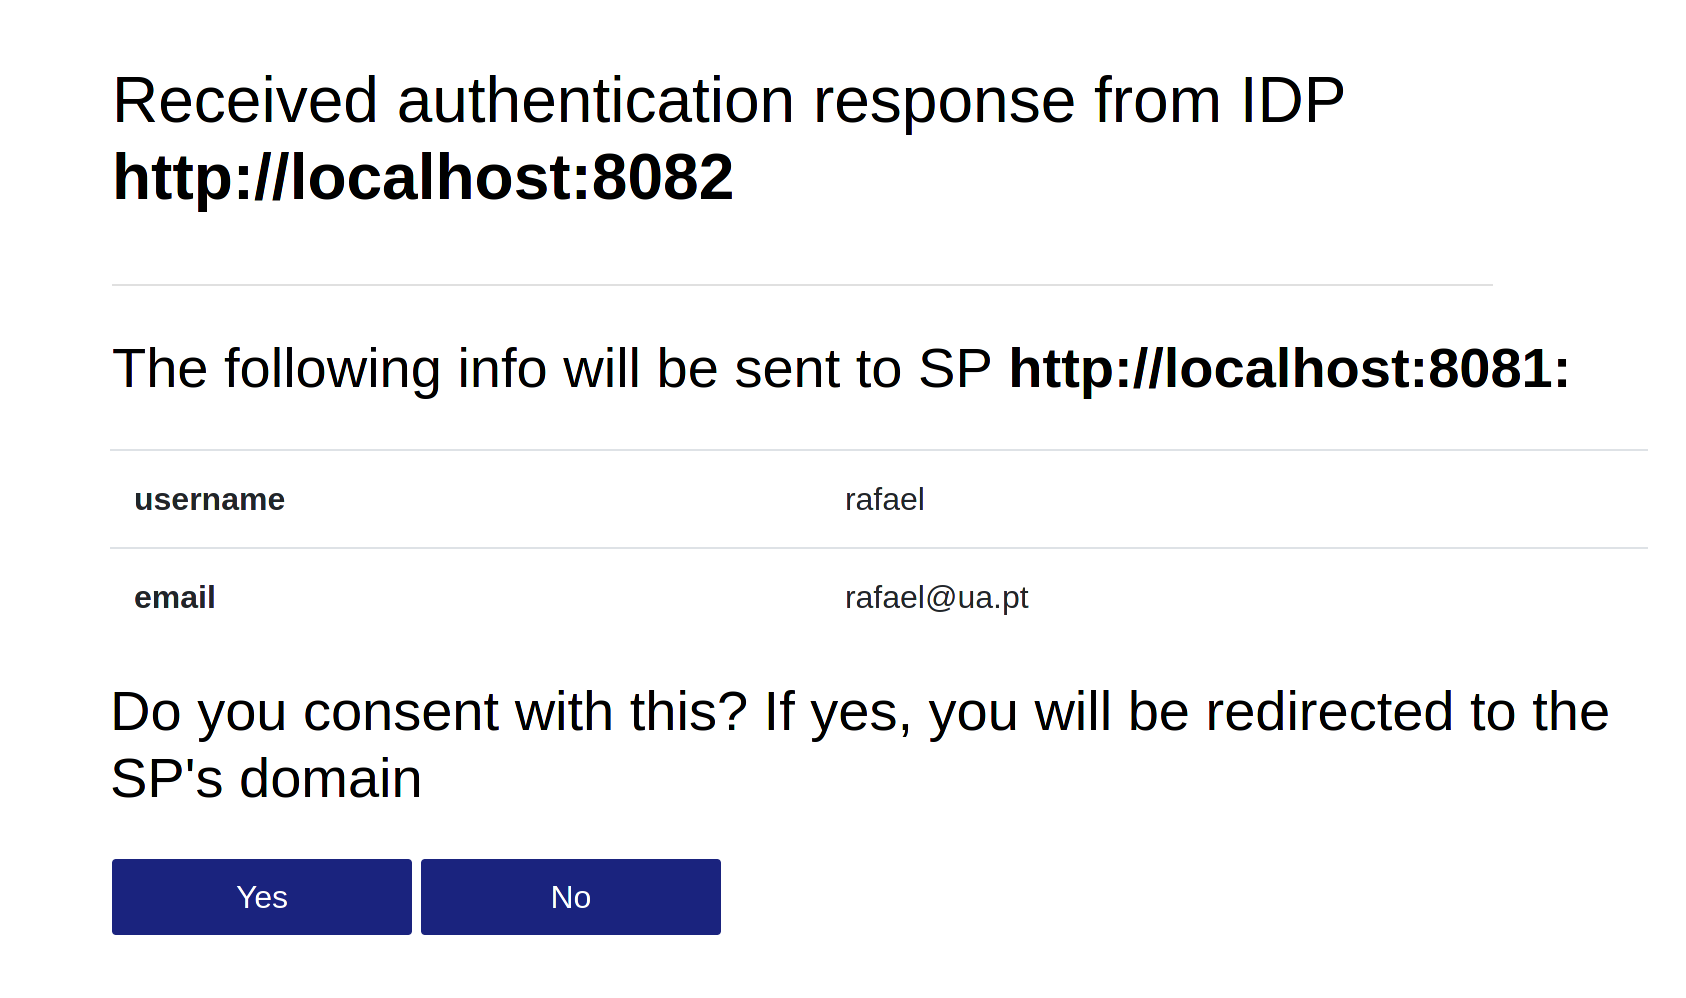
\includegraphics[width=0.6\textwidth]{img/response_conset.png}
        \centering
    \end{figure}
    \item Por fim, o \textit{SP} verifica a assinatura recebida com a chave publica do IDP e caso esta assinatura seja valida este consegue criar uma sessão para o utilizador usando os valores presentes na resposta recebida.
\end{enumerate}

\section{Extras}

\quad Nesta secção será relatado alguns mecanismos implementados para melhorar este caso de uso.

\subsection{Túnel seguro}

\quad Para garantir a proteção no intercâmbio de mensagens foi usado a mesma estratégia de criação de um túnel seguro implementado no primeiro projeto. No primeiro projeto isto foi possível pois o \textit{IDP} na primeira interação com o \textit{helper application} enviava um segredo partilhado para que ambas as entidades conseguissem cifrar as mensagens enviadas usando algoritmos de criptografia simétrica, contudo, neste novo serviço isto já não é possível pois já não existe esta primeira interação do \textit{idp} para a \textit{helper application}, portanto, para que este segredo seja criado e partilhado é necessário a \textit{helper application} fazer um operação explicita de obtenção deste segredo do \textit{IDP}. Portanto, antes de iniciar qualquer comunicação de autenticação e/ou processo de identificação a \textit{helper application} faz um \textit{redirect} para um \textit{endpoint} do \textit{IDP} que por sua vez redireciona novamente para a \textit{helper application} com o segredo partilhado enviado por argumento. Uma vez que estas operações de redirecionamento são seguras (devido ao uso de \textit{https}) a partilha do segredo é segura.






\end{document}
